\documentclass[12pt,a4paper]{article}

% Language setting
\usepackage[british]{babel}

% Set page size and margins
\usepackage[a4paper,top=2cm,bottom=2cm,left=2.5cm,right=2.5cm,marginparwidth=1.75cm]{geometry}

%----------- APA style references & citations (starting) ---
% Useful packages
%\usepackage[natbibapa]{apacite} % APA-style citations.

\usepackage[style=apa, backend=biber]{biblatex} % APA 7th edition style citations using biblatex
\addbibresource{references.bib} % Your .bib file

% Formatting DOI in APA-7 style
%\renewcommand{\doiprefix}{https://doi.org/}

% Add additional APA 7th edition requirements
\DeclareLanguageMapping{british}{british-apa} % Set language mapping
\DeclareFieldFormat[article]{volume}{\apanum{#1}} % Format volume number

% Modify 'and' to '&' in the bibliography
\renewcommand*{\finalnamedelim}{%
  \ifnumgreater{\value{liststop}}{2}{\finalandcomma}{}%
  \addspace\&\space}
  
%----------- APA style references & citations (ending) ---


\usepackage{amsmath}
\usepackage{graphicx}
\usepackage[colorlinks=true, allcolors=blue]{hyperref}
\usepackage{hyperref}
%\usepackage{orcidlink}
\usepackage[title]{appendix}
\usepackage{mathrsfs}
\usepackage{amsfonts}
\usepackage{booktabs} % For \toprule, \midrule, \botrule
\usepackage{caption}  % For \caption
\usepackage{threeparttable} % For table footnotes
\usepackage{algorithm}
\usepackage{algorithmicx}
\usepackage{algpseudocode}
\usepackage{listings}
\usepackage{enumitem}
\usepackage{chngcntr}
\usepackage{booktabs}
\usepackage{lipsum}
\usepackage{subcaption}
\usepackage{authblk}
\usepackage[T1]{fontenc}    % Font encoding
\usepackage{csquotes}       % Include csquotes
\usepackage{diagbox}


% Customize line spacing
\usepackage{setspace}
\onehalfspacing % 1.5 line spacing

% Redefine section and subsection numbering format
\usepackage{titlesec}
\titleformat{\section} % Redefine section numbering format
  {\normalfont\Large\bfseries}{\thesection.}{1em}{}
  
% Customize line numbering format to right-align line numbers
\usepackage{lineno} % Add the lineno package
\renewcommand\linenumberfont{\normalfont\scriptsize\sffamily\color{blue}}
\rightlinenumbers % Right-align line numbers

\linenumbers % Enable line numbering

% Define a new command for the fourth-level title.
\newcommand{\subsubsubsection}[1]{%
  \vspace{\baselineskip}% Add some space
  \noindent\textbf{#1\\}\quad% Adjust formatting as needed
}
% Change the position of the table caption above the table
\usepackage{float}   % for customizing caption position
\usepackage{caption} % for customizing caption format
\captionsetup[table]{position=top} % caption position for tables

% Define the unnumbered list
\makeatletter
\newenvironment{unlist}{%
  \begin{list}{}{%
    \setlength{\labelwidth}{0pt}%
    \setlength{\labelsep}{0pt}%
    \setlength{\leftmargin}{2em}%
    \setlength{\itemindent}{-2em}%
    \setlength{\topsep}{\medskipamount}%
    \setlength{\itemsep}{3pt}%
  }%
}{%
  \end{list}%
}
\makeatother

% Suppress the warning about \@parboxrestore
\pdfsuppresswarningpagegroup=1


%-------------------------------------------
% Paper Head
%-------------------------------------------
\title{Gaussian Process Boosting: Simulation Report}

\author[]{Yuqi YANG}
\affil[]{\small Hong Kong University of Science and Technology}
\affil[]{\texttt{yyangfd@connect.ust.hk}}

\date{}  % Remove date

\begin{document}
\maketitle

% \begin{abstract}
% Abstracts must be able to stand alone and so cannot contain citations to the paper’s references, equations, etc. An abstract must consist of a single paragraph and be concise. Because of online formatting, abstracts must appear as plain as possible. Three to six keywords must be included. Each keyword should not exceed three words. %\lipsum[1]
% \end{abstract}

% \textbf{Keywords}: keyword1, keyword2, keyword3, keyword4, keyword5, keyword6.  

{
  \hypersetup{linkcolor=black}
  \tableofcontents
}
\newpage

%-------------------------------------------
% Paper Body
%-------------------------------------------
%--- Section ---%
% \section*{Nomenclature}

% \begin{tabbing}
% $T$\qquad \= Temperature (K)\\
% $u_i$ \> Velocity in the x-direction (m/s)\\
% $\tau_{ij}$ \> Shear stress (N/m2)\\
% $\omega$ \> Specific turbulent dissipation rate (1/s)\\
% $Y_\omega$ \> Dissipation of $\omega$
% \end{tabbing}



%--- Section ---%
\section{Overview}

\subsection{Why is it interesting}

Standard boosting algorithm excels at solving complex non-linear modeling problems while staying robust over various scenarios in supervised learning settings. However, boosting algorithms always assume the independence relationships across different response variables when the predictors are given.

While Gaussian process, on the other hand, often starts with a zero or linear function prior assumption. Gaussian process or mixed effects modeling techniques can account for the residual correlations by design, but the prior assumption sometimes can be not necessarily correct and lead to a degradation of performance.

Therefore, these pros and cons of two different models call for a combined effort to model the possible intricate non-linearity and capture the residual correlations at the same time. This would be useful, and predictably, will achieve superior performance over stand-alone models. The results from the paper also have shown the feasibility and State-of-the-Art prediction accuracy of the proposed methodology.


\subsection{What are the major challenges to solve}

To combine the two models, we need to consider how to relax the constraint imposed by them. More specifically, we need to come up with a solution to relax both the linear prior or zero prior setting in mixed effects models and the independence setting in boosting architecture.

There have been literature trying to solve the problem in a three-step fashion:

\begin{enumerate}
  \item Use some learning algorithms to come up with a additive predictor function $f_{k+1}(\cdot)$
  \item In every iteration, try to estimate the covariance parameters
  \item In every iteration, try to estimate the random effects
\end{enumerate}

These procedures would work. However, the cost of computation is high, since in each round both step two and three requires recursive estimation and there would be rooms to optimize and level up the efficiency.


\subsection{How the proposed method solve the problem}

\subsubsection{Algorithm prototype}

We formalize our goal to minimizing the following loss function by choosing a suitable modeling function $F(\cdot)$ from the function space $\mathcal{H}$ for the boosting component, and suitable parameter $\theta$ from the covariance parameter space $\Theta$ of the Gaussian process, a negative log likelihood function is used as the loss function:
$$
\hat{F}, \hat{\theta} = {\arg\min}_{F, \theta \in \mathcal{H}, \Theta} L(y, F, \theta) \big|_{F = F(X)}
$$

\begin{algorithm}
\caption{\textit{Gaussian Process Boosting Prototype}}\label{alg:prototype}
\begin{algorithmic}[1]
\State \textbf{Input:} Initialized $\theta_0$, learning rate $\eta$, number of iterations $K$

\State Initialize $F_0() = \arg\min_{c \in \mathbb{R}} L(y, c\cdot \mathbb{I}, \theta_0)$
\For{$k = 1$ to $K$}
    \State Find $\theta_{k+1} = \arg\min_{\theta \in \Theta} L(y, F_{k}, \theta)$
    \State Conducting boosting step for finding the additive structure $f_{k+1}(\cdot)$
    \State Update $F_{k+1}(\cdot) = F_{k}(\cdot) + \eta f_{k+1}(\cdot)$
\EndFor

\State \textbf{return} Predictor function $\hat{F}(\cdot)$, covariance parameters $\hat{\theta}$
\end{algorithmic}
\end{algorithm}


\subsubsection{Update rule in the Boosting step}
When updating the predictor function $F(\cdot)$ in boosting, there are several choices available. One is using the Netwon step, which offers one-step of functional gradient followed by one-step optimization of parameters, and is therefore, efficient from the computational point of view:
$$
f_{k+1}(\cdot) = \arg\min_{f(\cdot)} (y - F_{k} - f)^T \Sigma_{k+1}^{-1} (y - F_{k} - f)
$$
but suffering from the overfitting problem, the boosting mechanisms often opt for an early stopping for the algorithm, which is not guaranteed to be optimally convergent. 

The alternative counterpart, known as the block descent technique, will optimize the function then parameter in an iterative manner, which would impose a great demand of computation, if we try to optimize both the function and parameter until the convergence condition is matched for the stopping of optimization in one iteration:
$$
f_{k+1}(\cdot) = \arg\min_{f(\cdot)} \| \Sigma_{k+1}^{-1} (F_{k} - y) - f \|^2
$$

Hence, inspired by both techniques, we could mitigate the inefficiency by opting for a fused updating rule: we use the Newton step to approximate the gradient of the function $F(\cdot)$ and then do a block descent, or coordinate descent to update the parameter $\theta$. In this manner, we would be more likely to achieve the optimal convergence while not compromising the overall efficiency. 


\subsubsection{Gaussian Process Boosting}

By joining the updating rule into the algorithm prototype, hence we get the vanilla Gaussian Process Boosting algorithm.

\begin{algorithm}
\caption{\textit{Gaussian Process Boosting}}\label{alg:vanilla_GPBoost}
\begin{algorithmic}[1]
\State \textbf{Input:} Initialized $\theta_0$, learning rate $\eta$, number of iterations $K$

\State Initialize $F_0() = \arg\min_{c \in \mathbb{R}} L(y, c\cdot \mathbb{I}, \theta_0)$
\For{$k = 1$ to $K$}
    \State Find $\theta_{k+1} = \arg\min_{\theta \in \Theta} L(y, F_{k}, \theta)$
    
    \State Find $\beta_{k+1} = \hat{\beta}$, $(\hat{\beta}, \hat{\nu}) = \arg\min_{(\beta, \nu): f() = h(;\beta)^T \nu \in \mathcal{S}} \| \Sigma_{k+1}^{-1} (F_{k} - y) - f \|^2$
    \State Calculate $\nu_{k+1} = (h_{\beta_{k+1}}^T \Sigma_{k+1}^{-1} h_{\beta_{k+1}})^{-1} h_{\beta_{k+1}}^T \Sigma_{k+1}^{-1} (y - F_{k})$
    \State Set $f_{k+1}() = h(;\beta_{k+1})^T \nu_{k+1}$
    
    \State Update $F_{k+1}(\cdot) = F_{k}(\cdot) + \eta f_{k+1}(\cdot)$
\EndFor

\State \textbf{return} Predictor function $\hat{F}(\cdot)$, covariance parameters $\hat{\theta}$
\end{algorithmic}
\end{algorithm}


%--- Section ---%
\section{Simulation Result\label{sec2}}
We conduct the simulation study based on the same setup as the simulated dataset mentioned in the Section 4.1\footnote{The overall methodology of the artificial derivation of the dataset is adopted while some of the hyper parameters could be different from the ones proposed in the paper.} of the paper (\cite{Sigrist2022}). The reproduced code can be found in the GitHub link provided below.\footnote{\url{https://github.com/AragornBFRer/GPBoost}}



\subsection{Simulation Setting}
We adopt the following mixed effects model with random effects $Zb$, both grouped mixed effects and Gaussian Process are incorporated under this setting: 
$$
y = F(X) + Zb + \epsilon, \quad b \sim \mathcal{N}(0, \Sigma), \quad \epsilon \sim \mathcal{N}(0, \sigma^2 I_n)
$$
a sample size of $n = 500$ for spatial dataset generated is used. The number is chosen to be relatively small to enable exact calculations during intermediate steps without doing large scale approximations.

To generate the spatial data, we use a exponential variance Gaussian process model, where the covariance function $k(s, s')$ is given by 
$$
k(s, s') = \sigma_1^2 \exp\left(-\frac{\|s - s'\|}{\rho}\right)
$$
here, the locations are constraint to be $[0,1]^2$ and $\rho = 0.1$. $\sigma_1^2 = 1$ is set as the marginal variance, and $\sigma^2 = 1$ as the error variance. By doing this, we can control the signal-to-noise ratio between the random effects $Zb$ and the error term $\epsilon$ to be 1.

For the fixed effects part, we consider the same simulation setting as the author referenced (\cite{Hajjem03062014}), where $F(x)$ is chosen to be 
$$
F(x) = C \cdot \left(2x_1 + x_2^2 + 4\mathbb{I}_{\{x_3>0\}} + 2 \log(|x_1|x_3) \right), \quad x = (x_1, \ldots, x_9)^{T}, \quad x \sim \mathcal{N}(0, I_9)
$$
here, $C$ is a normalization constant to control the variance of $F(x)$ to be approximately 1. In other words, the signal strength of the fixed effects part and the mixed effects part are about the same.

The dataset are split into different areas for training and testing purposes. For convenience, we term the testing dataset located in the same spot as the training dataset as the \textit{interpolation}, and the ones that are out of current training sample are termed as \textit{extrapolation}. In the spatial data setting we choose, the training data are sampled uniformly from $[0, 1]^2$ excluding $[0.5, 1]^2$. And the \textit{extrapolation} part are sampled uniformly from $[0.5, 1]^2$, as illustrated in Figure~\ref{fig:simulated_data}. The reproduction and implementation of the data simulator can be found in the corresponding GitHub link.\footnote{\url{https://github.com/AragornBFRer/GPBoost/tree/main/code}}


\begin{figure}
    \centering
    \includegraphics[width=0.6\textwidth]{figures/simulated_data.png}
    \caption{\small Demonstration of the simulated spatial data, where the \textit{training} set is sampled uniformly from $[0, 1]^2$ excluding $[0.5, 1]^2$, so as the \textit{interpolation} testing set. The \textit{extrapolation} testing set is simulated from $[0.5, 1]^2$, as shown in the reddish color. }
    \label{fig:simulated_data}
\end{figure}


\subsection{Empirical Results}

We carry out the comparison between the performance of proposed GPBoost model and the performance of \texttt{LightGBM} (\cite{Ke2017}) and \texttt{CatBoost} models.

As we can see from Figure~\ref{fig:GPB_hybrid}, the GPBoost outperforms LightGBM and CatBoost under the similar hyper parameter setting, showcasing the effectiveness of this algorithm. The result stays robust outside of current trained regions.\footnote{Note that the terming of \textit{extrapolation} and \textit{interpolation} is just for naming convenience, since it's "some sort of extrapolation" under spatial setting as the author suggests.}

We additionally visualize the solution path of the GPBoost algorithm and CatBoost algorithm as a comparative study. As shown in the Figure~\ref{fig:solution_path} below, the convergence speed of the proposed GPBoost algorithm is much faster than the CatBoost. This shows the superior efficiency of GPBoost under the hybrid updating step setting.

\begin{figure}
    \centering
    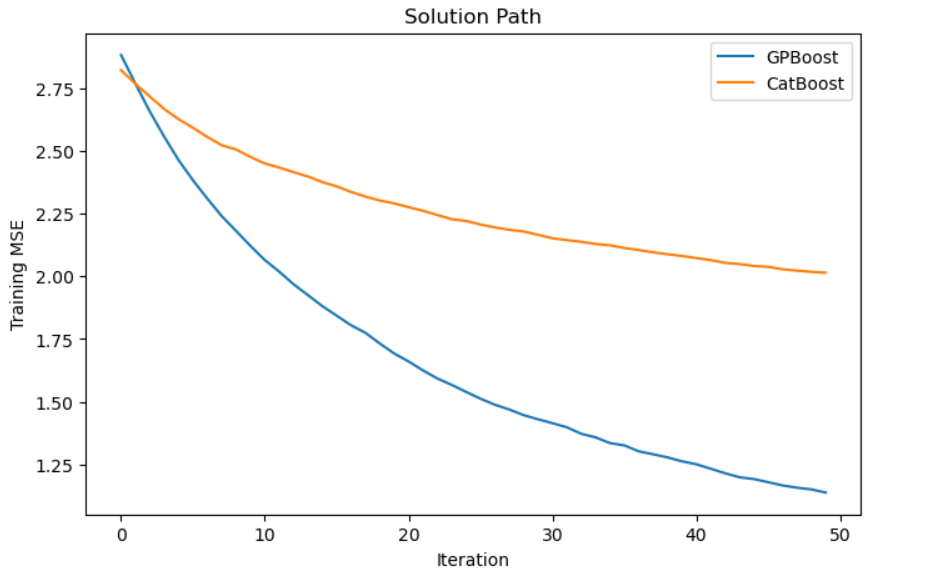
\includegraphics[width=0.7\textwidth]{figures/sol_path.png}
    \caption{\small This is the visualization of the solution path of GPBoost and CatBoost under the same number of iterations $num\_iter = 50$. }
    \label{fig:solution_path}
\end{figure}

\subsection{Ablation Study}

To testify the effectiveness and necessity of the proposed algorithm, we can adjust the types of updating rule used in the boosting step to see if the performance would change. As a result, the hybrid update step achieves the best performance under the above setting, while the demonstrated result in Figure~\ref{fig:GPB_grad} and Figure~\ref{fig:GPB_newton}, which used gradient algorithm and newton step for updating, appears to be worse. With hybrid step, the implemented algorithm can be better off compared to LightGBM and CatBoost model, while stand alone update rules may not.


\section{Conclusion}
The Gaussian Process Boosting model proposed in this paper cleverly combine the boosting structure with the mixed effects model to achieve better results for both individual models. The idea of relaxing both side of the assumptions to combine the models, i.e., relaxing the independence assumption in the boosting algorithm by introducing the correlated structures from the Gaussian Process model and relaxing the linear prior assumption of the mixed effects model via introducing non-linearity from the additive structure of boosting methods. This opens another realm of research thinking for me, to rethink the pros and cons of of each model from the bottom up, and exploit full potential of existing methods.


\section{Disclaimer}

I have used ChatGPT to facilitate my reproduction of the code. But I have not referred to other code sources. 


\begin{figure}
    \centering
    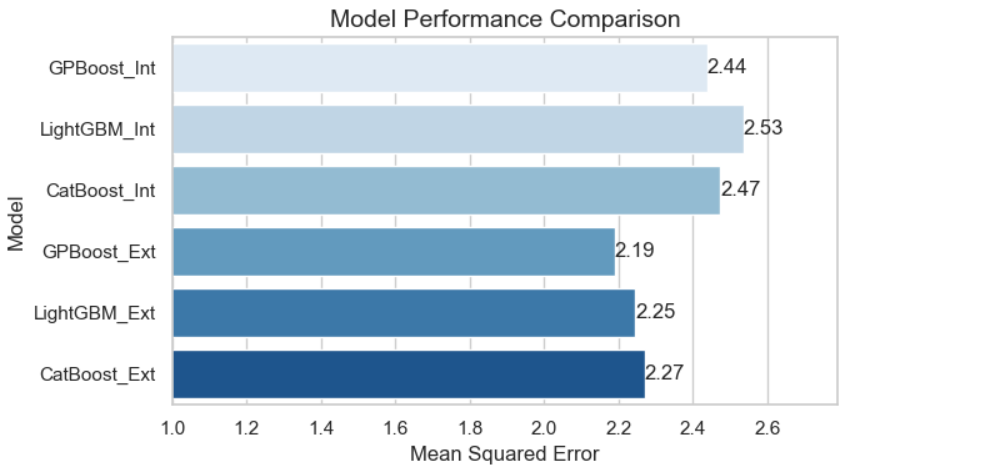
\includegraphics[width=1\textwidth]{figures/GPBoost_hybrid.png}
    \caption{\small Demonstration of the performance of GPBoost model with a hybrid of gradient algorithm and newton step used in the boosting step, measured in MSE. Where $\_Int$ stands for interpolation and $\_Ext$ stands for extrapolation. }
    \label{fig:GPB_hybrid}
\end{figure}

\begin{figure}
    \centering
    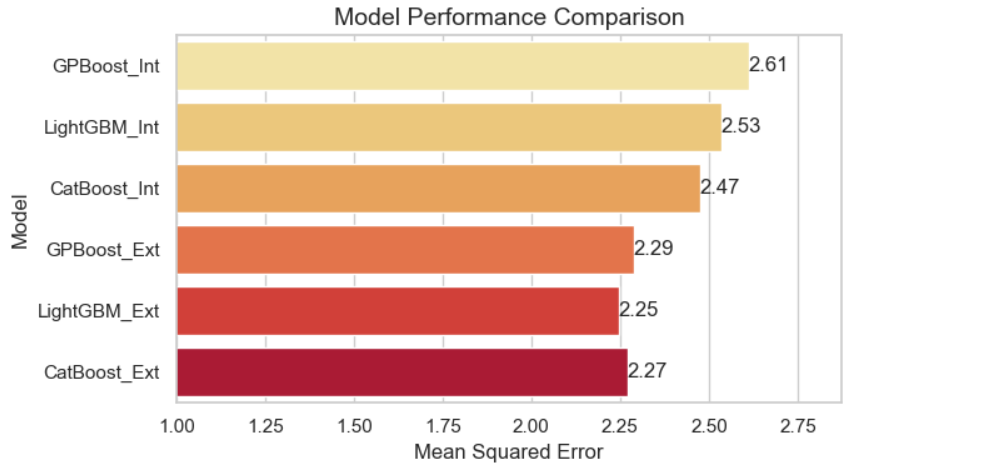
\includegraphics[width=1\textwidth]{figures/GPBoost_gradient.png}
    \caption{\small Demonstration of the performance of GPBoost model with gradient algorithm used in the boosting step, measured in MSE. Where $\_Int$ stands for interpolation and $\_Ext$ stands for extrapolation. }
    \label{fig:GPB_grad}
\end{figure}

\begin{figure}
    \centering
    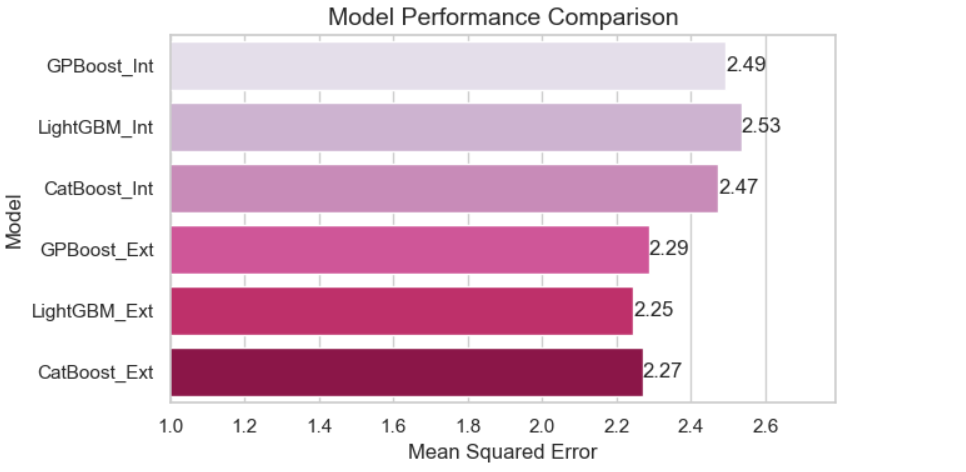
\includegraphics[width=1\textwidth]{figures/GPBoost_newton.png}
    \caption{\small Demonstration of the performance of GPBoost model with a newton step used in the boosting step, measured in MSE. Where $\_Int$ stands for interpolation and $\_Ext$ stands for extrapolation. }
    \label{fig:GPB_newton}
\end{figure}



%-------------------------------------------
% References
%-------------------------------------------

% Print bibliography
\printbibliography




%-------------------------------------------
% Appendix
%-------------------------------------------
% Activate the appendix in the doc
% from here on sections are numerated with capital letters 
%\appendix

% Change equation numbering format to be sequential within sections in the appendix
\renewcommand\theequation{\Alph{section}\arabic{equation}} % Redefine equation numbering format
\counterwithin*{equation}{section} % Number equations within sections
\renewcommand\thefigure{\Alph{section}\arabic{figure}} % Redefine equation numbering format
\counterwithin*{figure}{section} % Number equations within sections
\renewcommand\thetable{\Alph{section}\arabic{table}} % Redefine equation numbering format
\counterwithin*{table}{section} % Number equations within sections



\end{document}